\chapter{Background}
\label{chapter:background} 

\section{Overview}
This chapter focuses on the fundamental concepts for the rest of the chapters. We begin with introducing hybrid speech recognition systems and then compare them with end to end speech recognition systems in Section \ref{section:asr}. Then we discuss the different types of deep neural networks used in an \acrshort{asr} application. Finally, we discuss the SpeechBrain toolkit in Section \ref{section:sb}, which is used for all of our experiments.

\section{Speech Recognition}
\label{section:asr}

\subsection{Hybrid speech recognition systems}
%The terminology is a little unclear even in the field, but Hybrid mostly refers to HMM/DNN - but I guess what you're describing is more generally HMM based ASR. You can use this terminology too, cause nowadays HMM-based ASR is always HMM/DNN ASR; just be aware of the connotations.
\label{section:hybridasr}
Hybrid method of speech recognition use multiple steps which include feature generation, acoustic modelling and language modelling which combine to form a system which provides speech to text results. Figure \ref{fig:hyrid_asr_model} shows this architecture.

\begin{figure}[ht]
  \begin{center}
    % below the size of the figure has been reduced for example
    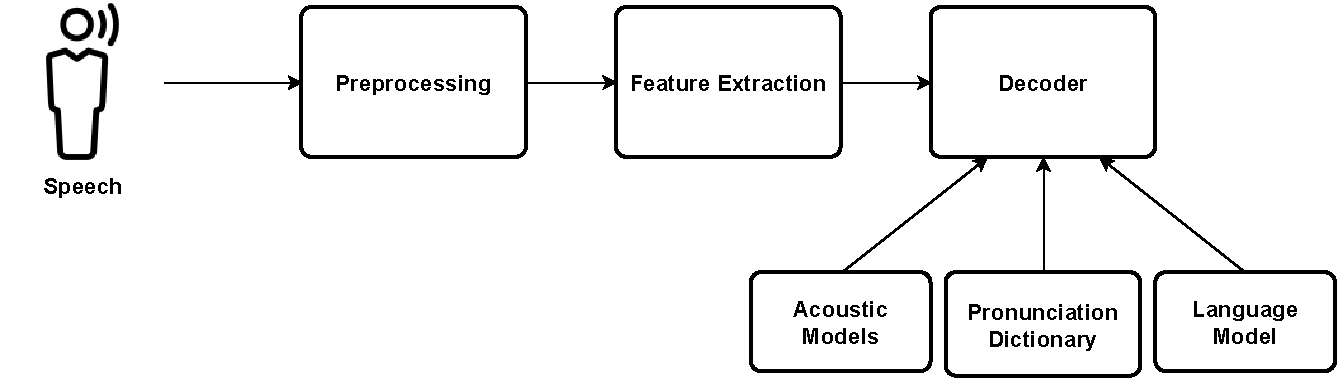
\includegraphics[width=\textwidth]{images/Hybrid ASR System.pdf} 
    \caption{A hybrid \acrshort{asr} system architecture}
    \label{fig:hyrid_asr_model}
  \end{center}
\end{figure}

In the \acrshort{hmm}-based architecture, the first step is preprocessing the speech signal to generate features which are robust to noise and convert the signal to vectors which are used in the decoder \cite{Mukhedkar2014RobustEnvironments}. The information of how different words are pronounced is stored in a pronunciation dictionary, also known as a lexicon. The goal of the decoder is finding the optimal word sequence, $\hat{\boldsymbol{W}}=W_{1}, W_{2}, \ldots, W_{m}$ with the number of words, $m$, is not known. This can be mathematically defined as maximizing the posterior probability $P(\boldsymbol{W} \mid \boldsymbol{O})$  \cite{Mansikkaniemi2010AcousticService}.

\begin{equation}
\begin{aligned}
\label{eqn:einstein} 
\hat{\boldsymbol{W}} &=\arg \max _{\boldsymbol{W}} P(\boldsymbol{W} \mid \boldsymbol{O}) \\
 &=\arg \max _{\boldsymbol{W}} \frac{P(\boldsymbol{O} \mid \boldsymbol{W}) P(\boldsymbol{W})}{P(\boldsymbol{O})} \\
 &=\arg \max _{\boldsymbol{W}} P(\boldsymbol{O} \mid \boldsymbol{W}) P(\boldsymbol{W}) 
\\ 
\end{aligned}
\end{equation}

Applying the Bayes rule on, $P(\boldsymbol{W} \mid \boldsymbol{O})$ we end up with the Equation \ref{eqn:einstein}, which is a combination of two probability models. $P(\boldsymbol{O} \mid \boldsymbol{W})$ corresponds to the acoustic model,  which computes the likelihood of the observed speech signal, given a possible word sequence and $P(\boldsymbol{W})$ corresponds to the language model \cite{Ney1999DynamicRecognition}. The language model represents our prior beliefs about what sequences of words are more or less likely. We say "prior" because this is knowledge that we have before we even process any speech signal. 


\subsection{End to end speech recognition systems}
\label{section:e2easr}
In end to end speech recognition systems, a single model, usually based on deep learning, replaces the hybrid \acrshort{asr} system stages. A deep learning model combined with an external language model can achieve higher performance than hybrid speech pipelines for particular applications \cite{Deshmukh2020ComparisonRecognition}. These systems rely on large neural networks, and as the size of the network grows and has millions of parameters, they require larger amounts of speech data to be trained well. Smaller models with lesser number of parameters can be trained with smaller amounts of data, but may fail to generalize well\cite{Tanaka2021End-to-EndLearning}. Since the system learns the whole task end-to-end, specialized components for capturing finer details of the speaker or other noise filtering components are not essential. On the contrary, previous experiments have shown that end to end models stand out in the cases where robustness is crucial\cite{Hannun2014DeepRecognition}. 

\section{What are Deep Neural Networks?}
A deep neural network is a neural network with many hidden layers. Deep neural networks can be trained to model non-linear models and functions for very high dimensional data \cite{Hammer2003AMachines}. Traditionally, it was quite challenging to train deep neural networks, but there was a resurgence in the usage of deep neural networks in the previous decade, also in the field of speech recognition \cite{Dahl2012Context-DependentRecognition, Morgan2012DeepRecognition, Deng2013RECENTMICROSOFT, Hannun2014DeepRecognition}. 

One of the first deep neural network was a \acrfull{mlp}, which consists of an input layer, an output layer and a hidden layer. Figure \ref{fig:mlp} shows this architecture. 

\begin{figure}[ht]
  \begin{center}
    % below the size of the figure has been reduced for example
    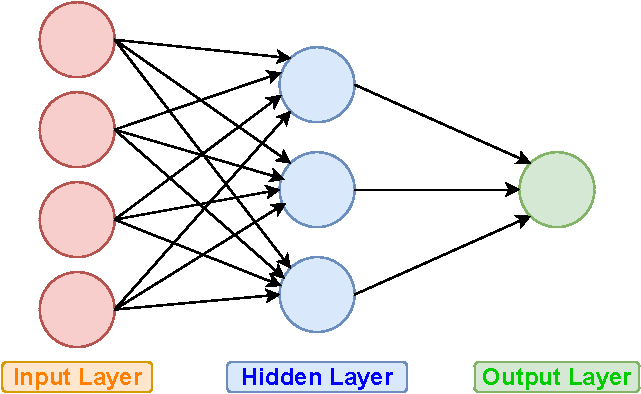
\includegraphics[width=\textwidth]{images/MLP.pdf} 
    \caption{An \acrshort{mlp} architecture}
    \label{fig:mlp}
  \end{center}
\end{figure}

Each layer of this network consists of multiple neurons, and each of these neurons can be represented using a vector, and all the neuronal connections in a layer can then be represented using a weights matrix that determines how much a neuron should take part in the decision-making process. At each layer, multiply the input signal with its corresponding weights and then add them up to obtain a weighed sum as the output of a layer. This can be represented as,

\[ z = w_1x_1 + w_2x_2 + .. + w_nx_n \]

In the above formula $z$ is the weighted sum output, $w$ is the weight, $x$ is an input and there are $n$ number of inputs. An activation function like tanh, sigmoid, ReLU, etc is applied to the weighted sum to get the output of the layer. 

\subsection{Model training}
Training of deep learning models use labelled data, split to train, validation and test splits. The model gradually learns to predict the labels of training data by adjusting the model weights based on the error. The validation split of the data is used to measure the accuracy of unseen data, periodically, during the training process. The test split, also unseen by the model, is not used during the process of training and used for evaluation of the different models after training them. The
most important metric studied is on the test data split \cite{Koliousis2019CROSSBOW:Servers}.

Let $w$ be a vector of model weights, and $x (w)$ be a loss function such that when given $y$, the ground truth and the predicted label $x$, measures the difference between them. Model training is an optimization problem that finds the best $w$ which minimizes the average loss over training data. In practice, this is accomplished using
\acrfull{sgd} \cite{Robbins1951AMethod}, an iterative algorithm that adapts $w$ using a few training samples at a time.

\begin{equation}
\label{eq:sgd}
\mathrm{w}_{n+1}=\mathrm{w}_{n}-\gamma_{n} \nabla \ell_{\mathrm{B}_{n}}\left(\mathrm{w}_{n}\right)
\end{equation}

where $\gamma_{n}$ is the learning rate in the $n$-th iteration of the algorithm, $\mathrm{B}_{n}$ is a mini-batch of $b$ training samples, and $\nabla \ell$ is the gradient of the loss function, averaged over the batch samples:
$$
\nabla \ell_{\mathrm{B}_{n}}\left(\mathrm{w}_{n}\right)=\frac{1}{b} \sum_{\mathrm{x} \in \mathrm{B}_{n}} \nabla \ell_{\mathrm{x}}\left(\mathrm{w}_{n}\right)
$$

The whole training process hence happens in two stages. First, a batch of labelled data propagates forward through the model to compute the output. This is compared to the ground-truth, measuring the loss value. Then, the error propagates backwards from the last layer to the first layer. This error is used to compute the gradient for the weights in each layer, and the weights can then be updated incrementally by applying Equation \ref{eq:sgd}.

When training such a deep learning model, the aim is to reduce time taken to achieve convergence with a target test accuracy results (time-to-benchmark). There are two factors which can affect the time-to-accuracy \cite{Koliousis2019CROSSBOW:Servers}.
\begin{enumerate}
    \item \textbf{Statistical Efficiency:} The number of iterations that a training algorithm such as SGD requires to find a solution with a given test accuracy. This can be done by optimizing the model architecture and improving the training data.
    \item  \textbf{Hardware Efficiency:} The execution time of each iteration. This can be done by improving and making maximum use of the computational infrastructure. 
\end{enumerate}

\emph{The focus of this thesis is hence to optimize the training by increasing the scale of data (statistical efficiency), while making maximum use of the available computational resources (hardware efficiency).} 
\newline

Next, we look at the deep neural network architectures that are used in this work. 
\subsection {Recurrent Neural Networks}
A \acrfull{rnn} is a type of neural network that can predict a future state by taking the previous states as input \cite{Graves2013SpeechNetworks}. This network can be thought of as having memory because it considers the context of the input provided to determine the output state \cite{Hagner2017RecurrentModel}.

Figure \ref{fig:rnn} represents the recurrent unit of an \acrshort{rnn}. It consists of an extra synapse that loops back into itself. In practise, this means that each unit receives a new input and also receives the output from the previous units as an input.
\begin{figure}[ht]
  \begin{center}
    % below the size of the figure has been reduced for example
    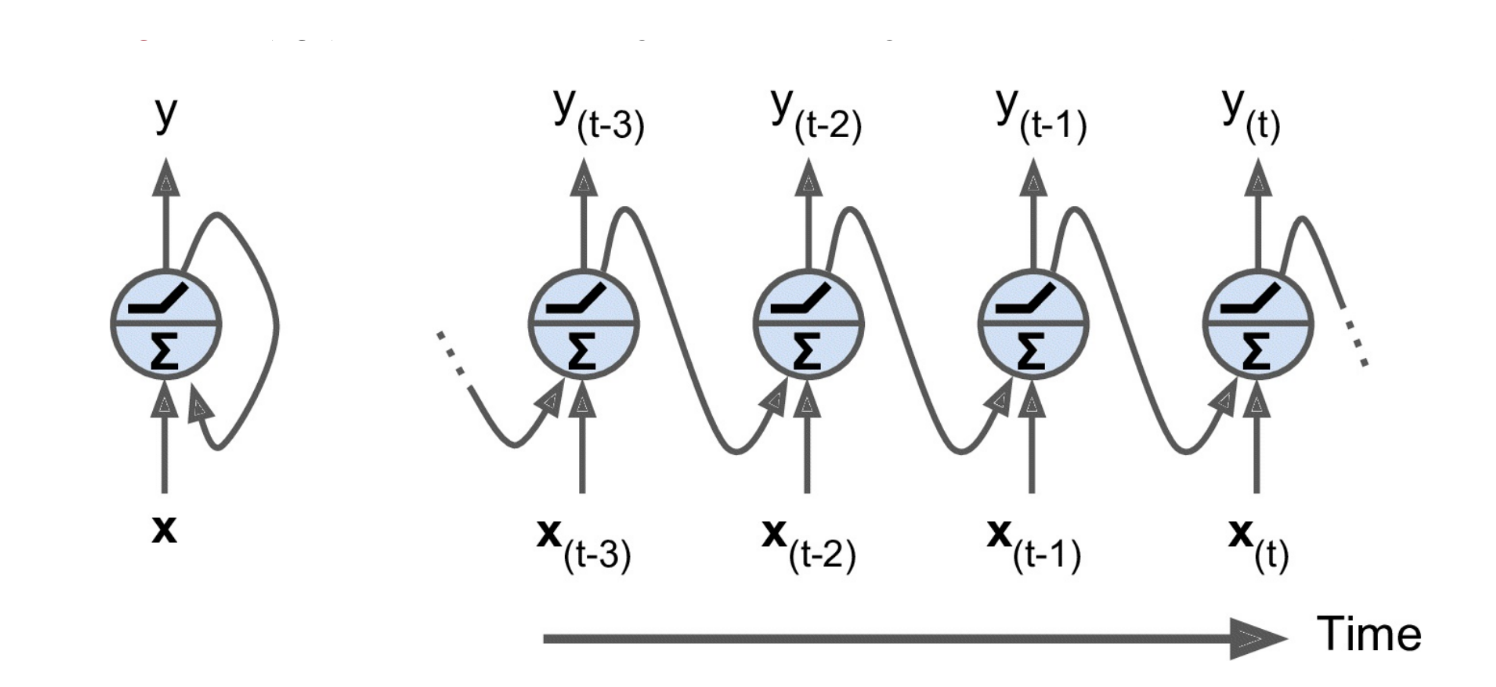
\includegraphics[width=\textwidth]{images/rnn.png} 
    \caption{A basic recurrent neural network cell and a way to visualize it
unrolling through time, from time step t-3 to t \cite{Hagner2017RecurrentModel}}
    \label{fig:rnn}
  \end{center}
\end{figure}

Consider an input series $\boldsymbol{x}=\left(x_{1}, \ldots, x_{T}\right)$, an \acrshort{rnn} calculates the hidden sequence $\boldsymbol{h}=\left(h_{1}, \ldots, h_{T}\right)$ and the output sequence $\boldsymbol{y}=$ $\left(y_{1}, \ldots, y_{T}\right)$ by looping the following equations from $t=1$ to $T$ :

$$
\begin{aligned}
&h_{t}=\mathcal{H}\left(w_{xh} x_{t}+w_{hh} h_{t-1}+b_{h}\right) \\
&y_{t}=w_{h y} h_{t}+b_{y}
\end{aligned}
$$

where the $w$ terms denote weight matrices, the $b$ terms denote bias vectors and $\mathcal{H}$ is the hidden layer function \cite{Graves2013SpeechNetworks}.

The drawback of an \acrshort{rnn} is that they use only the previous output to get the current context, but for speech recognition there is value to also utilize the future states too. A more advanced variation of \acrshort{rnn} is hence a \acrfull{brnn} \cite{Schuster1997BidirectionalNetworks}, which processes the input in both directions using two hidden layers and then this used as input to a single output layer. 

\subsubsection{Long Short-term Memory (LSTM)}
The main drawback with vanilla \acrshort{rnn}s is the vanishing gradient problem, which happens because the hidden states pass through a series of \inlinecode{tanh} activation functions, which leads to gradients becoming very close to zero and the network stops training through backpropagation \cite{Hochreiter1997LongMemory}. A \acrfull{lstm} cell \cite{Hochreiter1997LongMemory} modifies the \acrshort{rnn} architecture by passing another state vector to the next time step, along with the hidden state. The cell state variable enables the useful long term-based information to be preserved because this is modified only when there is new information. To control the cell state, gates which multiply a signal that is a continuous value ranging between 0 and 1 are used. Each gate has a weight matrix which are trained by iterating over the input data. The original work use two gates which are "input" gate, which control what information is essential and hence adds to the current state, and "output" gate which control what information needs to be written to the hidden state. More recently, a third gate called a "forget" gate controls deleting unwanted information from the cell state to stop cells growing in a boundless manner \cite{Gers2000LearningLSTM}.

\begin{figure}[ht]
  \begin{center}
    % below the size of the figure has been reduced for example
    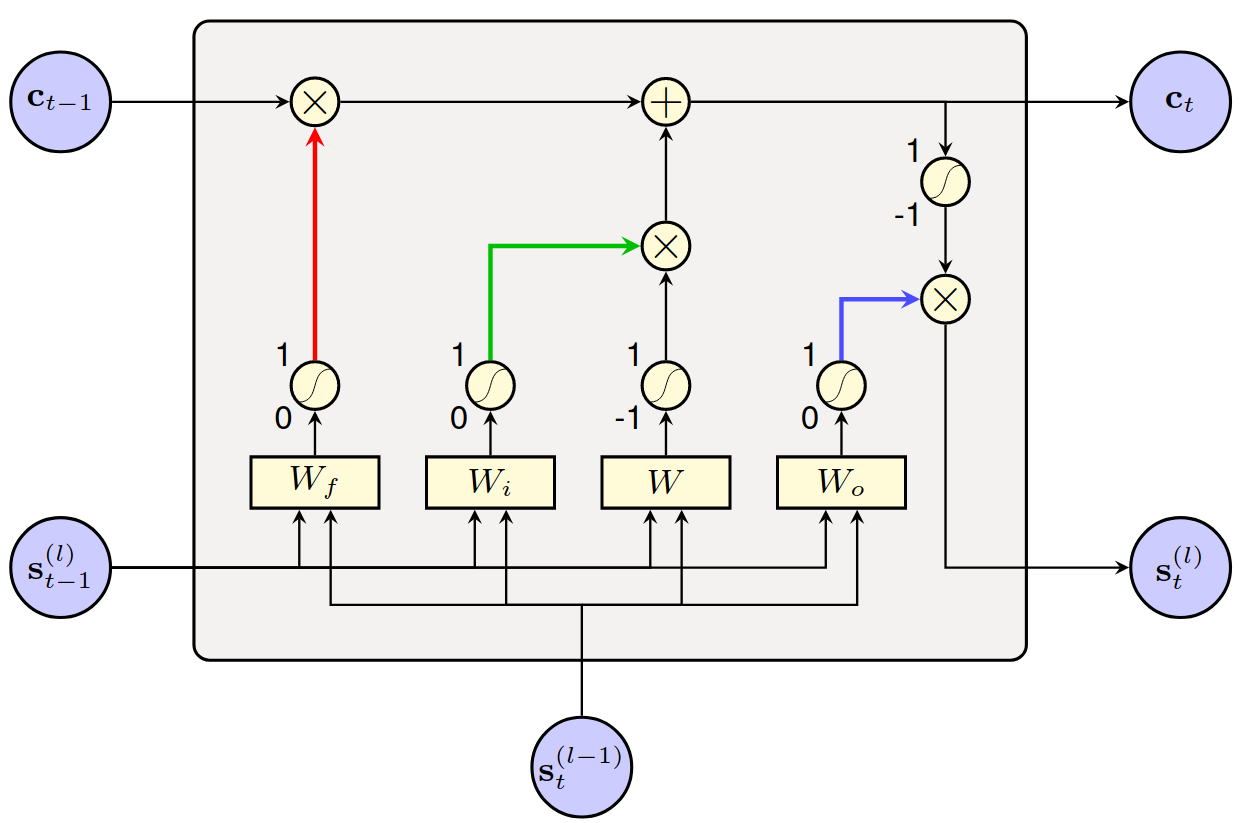
\includegraphics[width=\textwidth]{images/lstm.png} 
    \caption{A basic \acrshort{lstm} cell for a single time step \cite{Enarvi2018ModelingRecognition}}
    \label{fig:lstm}
  \end{center}
\end{figure}

Figure \ref{fig:lstm} shows the architecture of an \acrshort{lstm} layer with all the three gates. The three gates take in identical input, which also depends on the definition of the network. In most cases, the input to \acrshort{lstm} cell is the combination of the hidden state of the previous time step ($c_{t-1}$) and the output of the previous layer. Each gate contains 2 weight matrices, one each for the two inputs, and a bias vector. (Figure \ref{fig:lstm} shows only a weight matrix per gate.) 


\subsection {Convolutional Neural Networks}
\acrfull{cnn} is a branch of deep neural networks, which are hierarchical in nature and rely on convolution operations to process input. This helps to process data for tasks which can use spatial information by sharing the weights across the inputs. Hence, \acrshort{cnn}s  are especially powerful for performing tasks like image classification, object detection, etc on images and videos. \acrshort{cnn}s perform well when spatial features are important to perform the given task \cite{Krizhevsky2012ImageNetNetworks}.

The architecture of a general \acrshort{cnn} is alternating layers of convolution with subsampling layers \cite{Ciresan2011FlexibleClassification}. Figure \ref{fig:cnn} shows the architecture of AlexNet, one of the most popular \acrshort{cnn}s for image classification \cite{Krizhevsky2012ImageNetNetworks}. The architecture consists of convolutional layers altered with max pooling layers which act as sub sampling layers. The last layer of the network is using a fully connected layer to reduce the final dimensionality to match the required output shape.
\begin{figure}[ht]
  \begin{center}
    % below the size of the figure has been reduced for example
    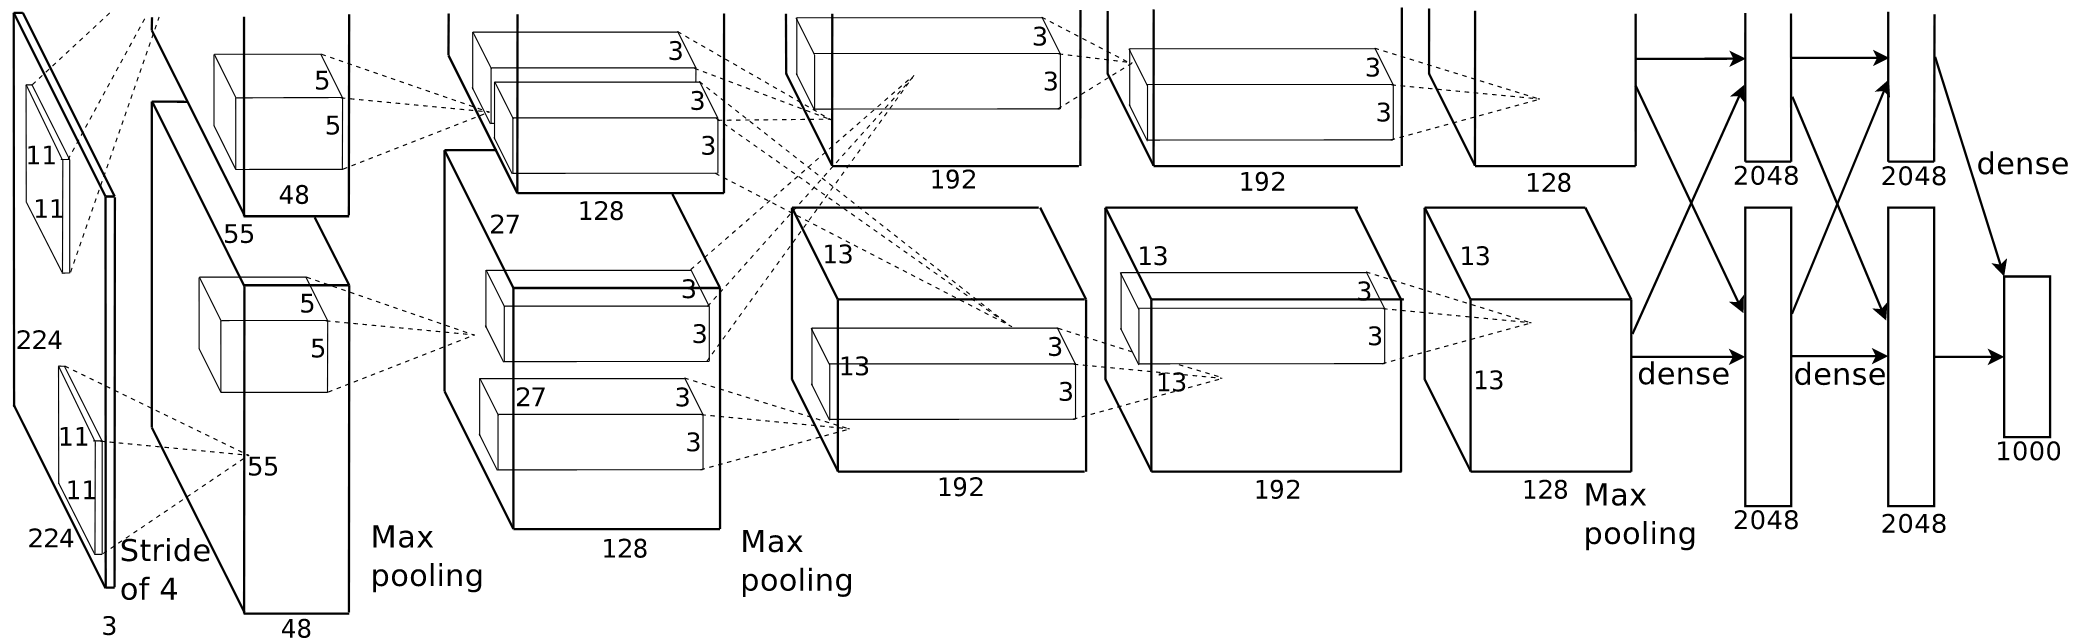
\includegraphics[width=\textwidth]{images/cnn.png} 
    \caption{AlexNet, a popular \acrshort{cnn} architecture  \cite{Krizhevsky2012ImageNetNetworks}}
    \label{fig:cnn}
  \end{center}
\end{figure}

More recently, convolutional neural networks have become popular for end to end speech recognition applications as well \cite{Zhang2017VeryRecognition}. The idea is to use convolutional layers along with a recurrent neural network. Unlike a typical \acrshort{rnn} with a fully connected layer, these networks replace it with a convolution layer because it is better at using the input topology to produce the output. These neural networks which are a combination of convolutional layers and a recurrent network are hence termed as \acrfull{crdnn}. 

\subsection {Atteniton-based Encoder Decoder (AED)}
Encoder-decoder type architecture models have become extremely popular over the last few years, and one of the variations in this branch of neural networks are the attention-based models \cite{Prabhavalkar2017ARecognition}. \acrfull{aed} models are a combination of two submodules: the Encoder module and the Decoder module. The encoder is an acoustic model which converts the input signal to an embedding representation. The decoder module takes the embeddings generated to produce a probability distribution for the output character sequences \cite{Zhang2017VeryRecognition, Chan2016ListenRecognition}.

\begin{figure}[ht]
  \begin{center}
    % below the size of the figure has been reduced for example
    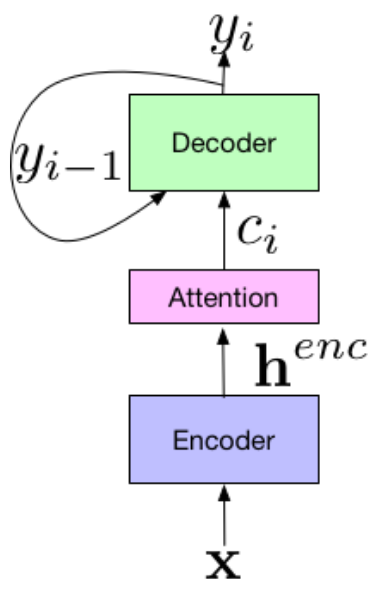
\includegraphics[width=0.3\textwidth]{images/las.png} 
    \caption{Architecture Diagram for a \acrshort{aed} model  \cite{Chiu2017State-of-the-artModels}}
    \label{fig:las}
  \end{center}
\end{figure}

Figure \ref{fig:las} represents the architecture of a \acrshort{aed} model with the encoder, attention, and decoder modules. The attention mechanism provides the context value. The below equations represents the functions in mathematical form.

$$
\begin{aligned}
\mathbf{h} &=\operatorname{Encoder}(\mathbf{x}) \\
P\left(y_{i} \mid \mathbf{x}, y_{<i}\right) &=\text {Decoder}\left(y_{<i}, \mathbf{h}\right)
\end{aligned}
$$
where $ \mathbf{h}$ is the embedding representation, the output from the encoder module and $P\left(y_{i} \mid \mathbf{x}, y_{<i}\right)$ represents the probability of the output character based on the input signal and the previous output characters.

Let $\mathbf{x}=\left(x_{1}, \ldots, x_{T}\right)$ be the input sequence and $\mathrm{y}$ be the output sequence of characters. \acrshort{aed} models produce for every character an output $y_{i}$ which is a conditional distribution based on the previously occurring sequence $y_{<i}$ and the original signal $\mathrm{x}$ by making use of the chain rule for probabilities:

$$
P(\mathbf{y} \mid \mathbf{x})=\prod_{i} P\left(y_{i} \mid \mathbf{x}, y_{<i}\right)
$$

This defines the end to end nature of the \acrshort{aed} models because it generates a probability distribution for the output characters sequence right from the input signal. 

\acrshort{aed} models output character scores for each sequence, and since datasets usually do not have character level alignments for speech data and their transcription. Training speech recognizers can become harder to train, than what it initially seems. To solve this issue, we use Connectionist Temporal Classification (CTC) loss to train \acrshort{aed} model.

\subsubsection{Connectionist Temporal Classification (CTC) Loss}
\label{section:ctc}
The \acrshort{ctc} criteria is a way of training end-to-end models when the target sequence and the input sequence do not match exactly in length. It eliminates the need to align the target labels on a frame to frame basis with the input training signal. When processing a speech that consists of the word ``to'', since the rate of speech varies from person to person, it is hard for the model to know the difference between ``toooooo'' or ``to''. We have to remove all duplicate ``o''s. But this will not work if the actual text required is ``too''? Then removing all duplicate ``o''s gets us the wrong result. \acrshort{ctc} loss helps to manage this.

From the previous encoder-decoder architecture, the difference is that the conditional probability of the output character at each time step, the encoder output embeddings $\mathbf{h}$, are then fed to a softmax layer which considers the whole set of blank-augmented output symbols to predict a probability distribution output similar in nature to the typical encode decoder output.


\section{SpeechBrain Toolkit}
\label{section:sb}
Speech recognition has always been driven forward due to the critical role played by open-source toolkits such as \acrshort{htk} \cite{Young2002TheBook}, Kaldi \cite{Povey2011TheToolkit}, etc. More recently, general purpose deep learning frameworks like TensorFlow \cite{Abadi2016TensorFlow:Systems} and PyTorch \cite{Paszke2019PyTorch:Library} have become useful for speech recognition tasks and this has led to newer toolkits like \acrshort{espnet} \cite{Watanabe2018ESPnet:Toolkit}. SpeechBrain \cite{Ravanelli2021SpeechBrain:Toolkit} is a toolkit designed to be flexible and used for multiple tasks to speed up research and development of speech related technologies.  SpeechBrain is a PyTorch-based toolkit and equipped to perform multiple tasks at once like recognize speech, understand its content, emotion, language, and speakers. 

\subsection{Brain class}
The SpeechBrain's core functionalities revolve around the \inlinecode{Brain} class, which defines a general training loop. The \inlinecode{Brain.fit()} method trains the models, and the Figure \ref{fig:brain} shows the basic components of the method. 

\begin{figure}[ht]
  \begin{center}
    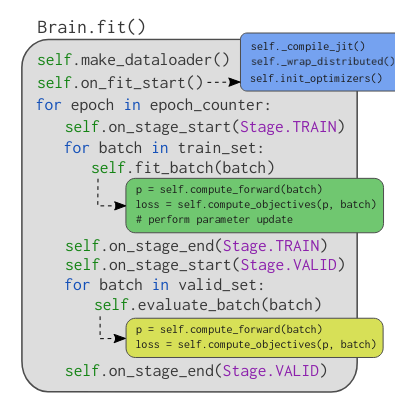
\includegraphics[width=0.5\textwidth]{images/brainclass.png} 
    \caption{\inlinecode{Brain.fit()} method illustration \cite{Ravanelli2021SpeechBrain:Toolkit}}
    \label{fig:brain}
  \end{center}
\end{figure}

Training of most \acrshort{dnn} models can be completed with a few lines of code. The Brain class also handles repetitive boilerplate code. It also calls the validation, learning rate scheduling, recoverable fault tolerant checkpointing modules. Training a model happens through a python script and run from the command line with the combination of a configuration file: 
\begin{verbatim} python train.py train.yaml\end{verbatim}

\subsection{HyperPyYAML}
The configuration file is in YAML format which is human-readable and can be used to define the model architecture, the data files, the parameters of the model, hyperparameters for training and other features of the pipeline. SpeechBrain utilities HyperPyYAML \footnote{speechbrain/HyperPyYAML:  Extensions  to  YAML  syntax  for  better python interaction. \href{https://github.com/speechbrain/HyperPyYAML}{https://github.com/speechbrain/HyperPyYAML} } which makes several extensions to the default YAML file format. The most important addition out of them is the easier object creation. An example:

\begin{verbatim}
epoch_counter: !new:speechbrain.utils.epoch_loop.EpochCounter
    limit: 100
\end{verbatim}

This tag with prefix \inlinecode{!new:} creates an instance of the specified class with an option to pass keyword arguments by using a mapping node like in the example above.

The next extension is the use of prefix, \inlinecode{!name} which simplifies the creation of an interface for specifying a function or class or other static Python entity. Below is an example using that.
\begin{verbatim}
opt_class: !name:torch.optim.Adam
    lr: !ref <lr>
\end{verbatim}
The prefix \inlinecode{!ref} is also an extension to the alias system used in YAML files. It takes keys in angles brackets and searched for the key within that YAML file. It can be used also for string interpolation, concatenation etc. It also has the \inlinecode{!include} prefix to import other YAML files to be used to reference in the current YAML file. This can be used to make the configuration files modular as well. 

\begin{verbatim}
dataset_parameters: !include:dataset.yaml
tokenizer_parameters: !include:tokenizer.yaml
\end{verbatim}

The last extension is the use of tuples. implicitly resolve any string starting with \inlinecode{(} and ending with \inlinecode{)} to a tuple.

\subsection{Other features}
SpeechBrain extends the PyTorch's data loading to help with speech data related challenges like handling variable length sequences and complicated data transformations. By leveraging PyTorch's \inlinecode{Dataset} and \inlinecode{DataLoader} classes, SpeechBrain enables on-the-fly data transformation (loading, augmentation, environment corruption, text processing, text encoding, feature extraction, etc) and can also be scaled to multiple parallel workers.

SpeechBrain also supports dynamic batching and multi \acrshort{gpu} training, which are discussed in detail in Chapter 4. This enables large-scale speech recognition tasks, which is the core of the work done in this thesis.  

SpeechBrain provides recipes for some of the most popular deep learning models and processing units which are used for different datasets. These can be used as is for the designed tasks, or they can also be modified to be used for custom tasks. This makes the development easier and initial bottleneck to start building ASR models is reduced.